\section{cSimple Module}
OMNet++ 모델은 Message를 주고받는 방식으로 communication 하는 modules로 구성되어 있다. 이때 사용되는 moudles는 각각 simple modules라고 정의되고 이번 보고서에서 조사하는 Simulation Class Library의 cpp로 작성되어 졌다. Figure 와 같이 simple modules 는 하나 또는 여러개로 group 지어서 compound modules를 구성할 수 있게 이때 규모의 제약없이 계층적인 구조를 형성할 수 있다. 이러한 모듈 전체를 OMNet++에서는 Network라고 하며 Network 그 자체 또한 compound module 이다.  이러한 연결에서 Message 는 서로 다른 modules 사이에서 전달이 된다. Figure에서 각 화살표가 connections 그리고 simple modules 내부에 있는 작은 상자가 gate를 나타낸다.\\
\vspace{-6mm}
\begin{figure}[h!]
\centering
\subfloat[\footnotesize Simple and Compound Modules ]{
    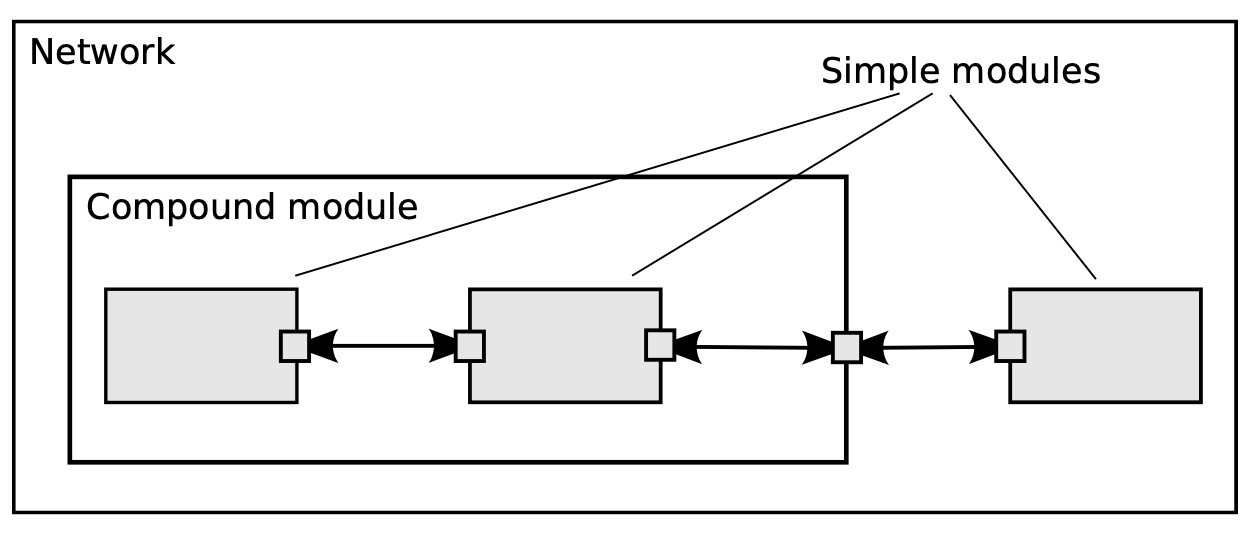
\includegraphics[width=0.7\textwidth] {image/week10/1-1.png}
}\hspace{5mm}
\subfloat[\footnotesize Inheritance of component]{
    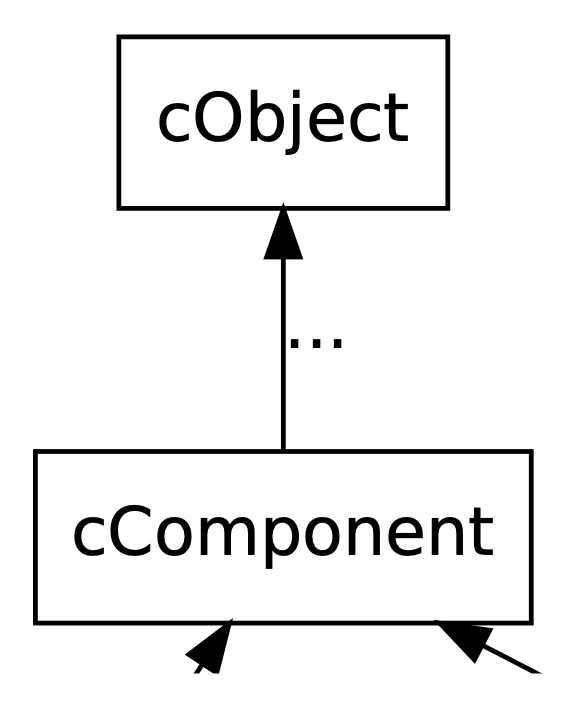
\includegraphics[width=0.23\textwidth] {image/week10/1-2.png}
}
\end{figure}

\vspace{-6mm}
\subsection*{cSimpleModule}
이번 실험에서 사용하는 OMNet++의 시뮬레이션 모델은 모듈과 연결로 구성된다. Figure (a)에 해당되는 single, compound 모듈들과 그 모듈간의 연결로 이해할 수 있다.
Simulatioin Library 에서 모듈과 채널은 각각 cModule, cChannel의 class로 표시된다. 이떄 cModule 과 cChannel 모두 cComponent Class 에서 파생된다.

cSimpleModule은 네트워크 시뮬레이션을 진행하기 위해 Compound Module을 구성해준 각각의 instance된 cComponents들을 cSimpleModule의 subclassing 방식으로 User가 NED 파일의 @class로 재정의하는 방법으로 구성이 가능하도록 해준다.
\subsection*{Sending Message}
Modules는 임의의 모든 데이터를 담을 수 있는 Message를 이용해 communicate 한다. Simple Modules 는 일반적으로 gates를 통해서 Message를 보내지만  다른 Module의 dsetination으로 직접 Message를 전달하는 것  또한 가능하다. 
    \subsubsection*{\mintinline{c}{send(cMessage *msg, const char *gateName, int index=0)}}
    Message 객체가 생성이 되면 output gate를 통해서 다른 module로 전송한다. 
\vspace{-2mm}
    \subsubsection*{\mintinline{c}{sendDirect(cMessage *msg, cModule *mod, int gateId)}}
    네트워크를 구성할때 \mintinline{c}{send()}와 같이 일반적으로 output gate를 거쳐 보내는것 외에, 직접 다른 모듈의 input gate로 전송할때 \mintinline{c}{sendDirect()}를 사용한다. 즉 직접적인 connection 이 없는 module 사이에서만 사용이 가능하다.
\vspace{-2mm}
\subsection*{Self-Message, Scheduling an Event}
Module은 자신에게 \mintinline{c}{scheduleAt()} function 을 사용해서 Message를 보낼 수 있다.
    \subsubsection*{\mintinline{c}{scheduleAt(t, msg)}}
    function에서 사용되는 parameter \mintinline{c}{t} 는 시뮬레이션상의 \textit{absolute time} 이다. 추가로 이렇게 보내지는 self-message는 다른 message 들과 동일한 방법으로 module에 도착하고, 필요하다면 \mintinline{c}{isSelfMessage()}로 확인이 가능하다.
\vspace{-2mm}
\subsection*{Components}
앞서 다룬것과 같이 cSimpleModule에서 네트워크 시뮬레이션을 위해 cComponents 로 instance 화된 module들을 아래의 cSimpleModule의 member function들이 repackaging을 관장한다. 
    \subsubsection*{initialize()}
    이 함수는 OMNeT++가 네트워크를 설정한 후에 호출되며\footnote{즉, 모듈을 만들고 정의에 따라 연결}, 초기화 코드를 위한 장소를 제공한다.
\vspace{-2mm}
    \subsubsection*{handleMessage(cMessage *msg)}
    OMNeT++에서 이벤트는 Simple Module 내부에서 발생한다. Simple Module은 이벤트를 생성하고 이벤트에 반응하는 C++ 코드를 encapulate 해서 module의 동작을 implement 해주는데, 이러한 동작인 동작을 정의해주기 위해 cSimpleModule의 member finction을 통헤 override 해주어야 한다.\\
    그중 module이 메세지를 수신하는 과정에서 message를 parameter로 호출이 되는데 \mintinline{c}{handlemessage()}를 통해서 처리되고 return 되는 과정을 거친다.\\
\vspace{-4mm}  
    \begin{figure}[!h]\centering
		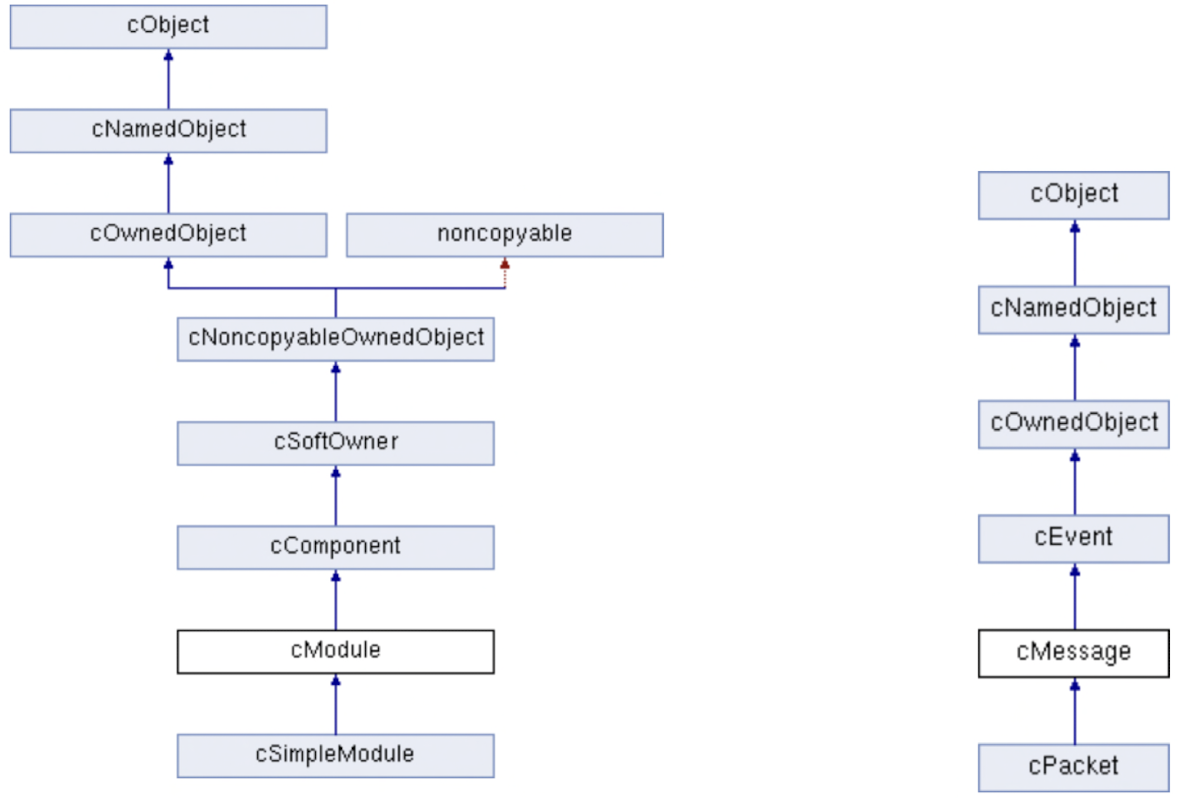
\includegraphics[width=.7\textwidth]{image/week10/23.png}
		\caption*{\small Inheritnace diagram for cModile \& cMessage}
		\vspace{-10pt}
    \end{figure}
\vspace{-4mm}